\documentclass[12pt,a4paper]{article}
\usepackage[T1,T2A]{fontenc}
\usepackage[utf8]{inputenc}
\usepackage[english,russian]{babel}
\usepackage{microtype}
\usepackage{csquotes}
\usepackage{amsmath}
\usepackage{amsthm}
\usepackage{amssymb}
\usepackage{mathtext}
\usepackage[notrig,italicdiff]{physics}
\usepackage{newfloat}
\usepackage{caption}
\usepackage{indentfirst}
\usepackage{geometry}
\usepackage{hyperref}
\usepackage{mdframed}
\usepackage[inline]{enumitem}
\usepackage{graphicx}
\usepackage{subfig}
\usepackage{titlesec,titletoc}
\usepackage[titletoc,title]{appendix}
\geometry{left=3cm,right=2cm,top=2cm,bottom=2cm}
\DeclareGraphicsExtensions{.pdf,.png,.jpg,.PNG}
\graphicspath{{./img/}}
\captionsetup[figure]{justification=centering}
\renewcommand{\thesubfigure}{\asbuk{subfigure}}
\DeclareCaptionLabelSeparator{dotseparator}{. }
\titlelabel{\thetitle. }
\patchcmd{\appendices}{\quad}{. }{}{}
\captionsetup{labelsep=dotseparator}
\hypersetup{
	colorlinks,
	citecolor=black,
	filecolor=black,
	linkcolor=black,
	urlcolor=black
}

\begin{document}

    \newcommand\blanktextfield[2]{$\underset{\text{#1}}{\text{\underline{\hspace{#2}}}}$}

\makeatletter
\begin{titlepage}

	\large\newpage

    \noindent\centering{
    	МИНИСТЕРСТВО ОБРАЗОВАНИЯ И НАУКИ РОССИЙСКОЙ ФЕДЕРАЦИИ

    	Федеральное государственное автономное образовательное учреждение высшего образования \enquote{Национальный исследовательский Нижегородский государственный университет им. Н.И. Лобачевского}
    }

	\vspace*{50pt}

	Физический факультет \\[\baselineskip]

	Кафедра информационных технологий\\
	в физических исследованиях

	\vspace*{\fill}

	{\Large\textbf{Модель Изинга на квадратной решетке для ферромагнетика с переворотом спина в каноническом ансамбле}}

	\vspace*{\fill}

	\hfill\begin{minipage}{22em}
    	Отчет по лабораторной работе\\
		студента 1 курса магистратуры 05182 группы\\
		\textbf{Василевского А.В.}
    \end{minipage} \\[\baselineskip]

	\hfill\begin{minipage}{22em}
		Основная профессиональная образовательная
		программа подготовки магистров по
		направлению 09.04.02~--- \enquote{Информационные системы и технологии}
		(профиль программы: \enquote{Информационные системы и технологии в физических исследованиях})
    \end{minipage}

	\vspace*{\fill}

	\hfill\begin{minipage}{15em}
		\blanktextfield{(подпись)}{1in} Василевский А.В.\\[\baselineskip]
		Руководитель учебной практики:\\
		доцент кафедры ИТФИ\\
		к. ф.-м. н.\\[\baselineskip]
		\blanktextfield{(подпись)}{1in} Васин А.С.
    \end{minipage}

	\vspace*{\fill}

	Нижний Новгород\\
	2018

\end{titlepage}
\makeatother


    \tableofcontents

    \clearpage

    %
    %
    %
    %%%%%%%%%%%%%%%%%%%%%%%%%%%%%%%%%%%%%%%%%%%%%%%%%%%%%%%%%%%%%%%%%%%%%%%
    %                           SECTION                                   %
    %%%%%%%%%%%%%%%%%%%%%%%%%%%%%%%%%%%%%%%%%%%%%%%%%%%%%%%%%%%%%%%%%%%%%%%
    %
    %
    %

    \section{Постановка задачи}

        Исследовать зависимость энергии, намагниченности, теплоемкость и магнитной восприимчивости ферромагнетика (антиферромагнетика) от температуры с использованием модели Изинга с переворачиванием спинов.

    %
    %
    %
    %%%%%%%%%%%%%%%%%%%%%%%%%%%%%%%%%%%%%%%%%%%%%%%%%%%%%%%%%%%%%%%%%%%%%%%
    %                           SECTION                                   %
    %%%%%%%%%%%%%%%%%%%%%%%%%%%%%%%%%%%%%%%%%%%%%%%%%%%%%%%%%%%%%%%%%%%%%%%
    %
    %
    %

    \section{Физическая модель}

        Будем рассматривать некоторый объем прямоугольной формы однородного ферромагнетика (антиферромагнетика) в двумерном пространстве. В качестве граничных условий используем периодические. Будем считать, что спины располагаются в каждом узле прямоугольной равномерной сетки. Динамику спинов будем описывать при в модели Изинга с переворотом спина.

    %
    %
    %
    %%%%%%%%%%%%%%%%%%%%%%%%%%%%%%%%%%%%%%%%%%%%%%%%%%%%%%%%%%%%%%%%%%%%%%%
    %                           SECTION                                   %
    %%%%%%%%%%%%%%%%%%%%%%%%%%%%%%%%%%%%%%%%%%%%%%%%%%%%%%%%%%%%%%%%%%%%%%%
    %
    %
    %

    \section{Математическая модель}

        %
        %
        %
        %%%%%%%%%%%%%%%%%%%%%%%%%%%%%%%%%%%%%%%%%%%%%%%%%%%%%%%%%%%%%%%%%%%
        %                        SUBSECTION                               %
        %%%%%%%%%%%%%%%%%%%%%%%%%%%%%%%%%%%%%%%%%%%%%%%%%%%%%%%%%%%%%%%%%%%
        %
        %
        %

        \subsection{Модель Изинга}

            Модель Изинга~--- простейшая модель фазовых взаимодействий в магнетике. Опишем модель Изинга в простейшей постановке.

            Рассмотрим решетку, содержащую $N$ узлов. Свяжем с каждым узлом спиновое число $s_i=\pm 1$. Набор чисел ${s_i} \forall i \in [1,N]$ будем называть состоянием системы. Нам интересны макроскопические характеристики системы: средняя энергия, средняя намагниченность, теплоемкость, магнитная восприимчивость, температура фазового перехода и т.д.

            Энергия описанной системы определится выражением
            %
            \begin{equation*}
                E = -J \sum\limits_{i,j=1}^N s_i s_j .
            \end{equation*}
            %
            Константа обменного взаимодействия $J$ является мерой силой взаимодействия между ближайшими соседними спинами.

            Намагниченность выражается проще
            %
            \begin{equation*}
                M = \qty|\frac{n_{+} - n_{-}}{N^2}| .
            \end{equation*}
            %
            Здесь $n_{\pm}$~--- количество положительных (отрицательных) спинов в области.

            Теплоемкость и восприимчивость на спин можно вычислить следующим образом через средние:
            %
            \begin{equation*}
                C = \frac{1}{N^2} \frac{1}{k^2 T^2} \qty(\left<E^2\right> - \left<E\right>^2), \quad
                \chi = \frac{1}{N^2} \frac{1}{kT} \qty(\left<M^2\right> - \left<M\right>^2) .
            \end{equation*}

            Температуру фазового перехода можно определить как точку экстремума $C(T)$. Из теории же известно, что
            %
            \begin{equation*}
                T_c = \frac{J}{k} \frac{2}{\ln(1+\sqrt{2})} .
            \end{equation*}

            В двумерной модели Изинга полезно использовать периодические граничные условия.

        %
        %
        %
        %%%%%%%%%%%%%%%%%%%%%%%%%%%%%%%%%%%%%%%%%%%%%%%%%%%%%%%%%%%%%%%%%%%
        %                        SUBSECTION                               %
        %%%%%%%%%%%%%%%%%%%%%%%%%%%%%%%%%%%%%%%%%%%%%%%%%%%%%%%%%%%%%%%%%%%
        %
        %
        %

        \subsection{Динамика модели Изинга}

            Будем рассматривать модель Изинга с динамикой с переворотом спина. Опишем алгоритм изменения конфигурации системы, основанный на алгоритме Метрополиса.
            %
            \begin{enumerate}[nosep]
                \item Генерируется начальное состояние системы $S$. Приемлемым вариантом является случайное равномерное распределение спинов разных знаков.
                \item Конфигурация $S'$ получается из $S$ переворотом случайно выбранного спина.
                \item Вычисляется изменение энергии системы $\Delta E = E(S') - E(S)$.
                \item Если $\Delta E < 0$, то состояние $S'$ принимается: $S \longleftarrow S'$.
                \item В противном случае состояние $S'$ может быть принято только по вероятности. Для этого генерируется случайное равномерно распределенное число $R \in [0,1]$.
                \item \begin{enumerate}
                    \item Если $R < \exp(\flatfrac{\Delta E}{kT})$, то состояние $S'$ принимается: $S \longleftarrow S'$.
                    \item Иначе состояние $S'$ отвергается.
                \end{enumerate}
            \end{enumerate}
            %
            Единицей времени в алгоритме служит один шаг Монте-Карло: $N$ итераций данного алгоритма.

            Оценку макроскопических характеристик следует производить после установления стационарного режима в системе, т.е. после по крайней мере нескольких сотен (тысяч) временных шагов.

    %
    %
    %
    %%%%%%%%%%%%%%%%%%%%%%%%%%%%%%%%%%%%%%%%%%%%%%%%%%%%%%%%%%%%%%%%%%%%%%%
    %                           SECTION                                   %
    %%%%%%%%%%%%%%%%%%%%%%%%%%%%%%%%%%%%%%%%%%%%%%%%%%%%%%%%%%%%%%%%%%%%%%%
    %
    %
    %

    \section{Анализ результатов}

        В ходе работы была написана демонстрационная программа (\autoref{fig:mainwindow}) на языке  \enquote{C++}, позволяющая наглядно исследовать динамику модели при фиксированной температуре, и в зависимости от температуры, а также определить макроскопические характеристики системы (энергия, намагниченность, теплоемкость, восприимчивость, температура фазового перехода).
        %
        \begin{figure}[h]
            \centering
            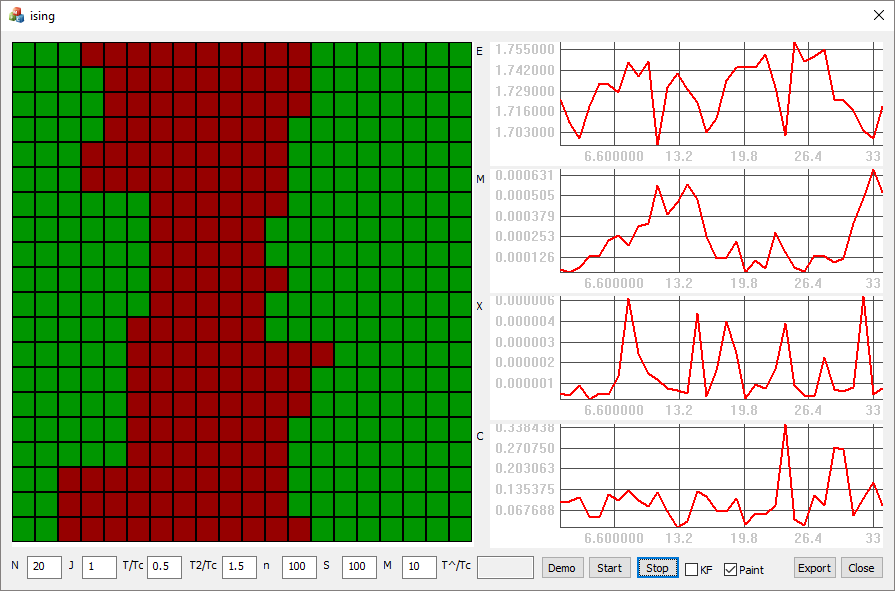
\includegraphics[width=0.8\textwidth]{mainwindow}
            \caption[]{Главное окно программы}
            \label{fig:mainwindow}
        \end{figure}
        %
        Два знака спина обозначается двумя разными цветами ячейки.

        На \autoref{fig:1}-\autoref{fig:3} представлены полученные стационарные состояния системы при разных температурах и разных размерах области моделирования. Следует отметить, что при все большем значении $N$ картина распределения спинов фактически лишь увеличивается в размере. К тому же, уместить ее на бумаге становится сложнее. Потому здесь мы ограничились предельным случаем $N = 100 \times 100$, когда картина еще не сливается в единое \enquote{пятно}.
        %
        \begin{figure}[!htb]%
            \centering
            %
            \subfloat[][]{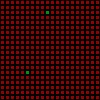
\includegraphics[width=0.25\textwidth]{board20_05}}%
            \hspace{8pt}%
            %
            \subfloat[][]{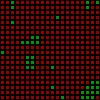
\includegraphics[width=0.25\textwidth]{board20_10}}%
            \hspace{8pt}%
            %
            \subfloat[][]{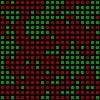
\includegraphics[width=0.25\textwidth]{board20_15}}%
            \hspace{8pt}%
            %
            \subfloat[][]{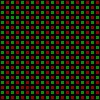
\includegraphics[width=0.25\textwidth]{boardi20_05}}%
            \hspace{8pt}%
            %
            \subfloat[][]{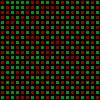
\includegraphics[width=0.25\textwidth]{boardi20_10}}%
            \hspace{8pt}%
            %
            \subfloat[][]{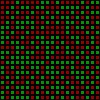
\includegraphics[width=0.25\textwidth]{boardi20_15}}%
            \hspace{8pt}%
            %
            \caption[]{Картины распределения спинов при $N=20\times 20$ для ферро- и антиферромагнетика.}%
            \label{fig:1}%
        \end{figure}
        %
        \begin{figure}[!htb]%
            \centering
            %
            \subfloat[][]{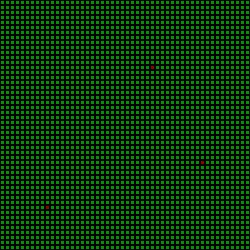
\includegraphics[width=0.25\textwidth]{board50_05}}%
            \hspace{8pt}%
            %
            \subfloat[][]{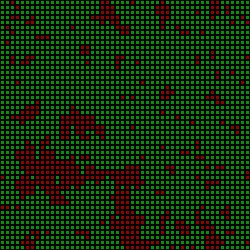
\includegraphics[width=0.25\textwidth]{board50_10}}%
            \hspace{8pt}%
            %
            \subfloat[][]{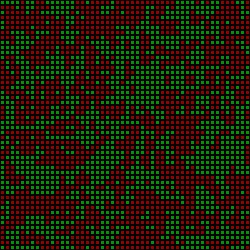
\includegraphics[width=0.25\textwidth]{board50_15}}%
            \hspace{8pt}%
            %
            \subfloat[][]{
\includegraphics[width=0.25\textwidth]{boardi50_05}}%
            \hspace{8pt}%
            %
            \subfloat[][]{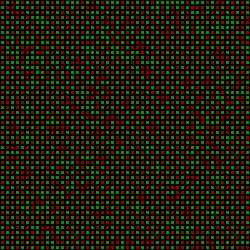
\includegraphics[width=0.25\textwidth]{boardi50_10}}%
            \hspace{8pt}%
            %
            \subfloat[][]{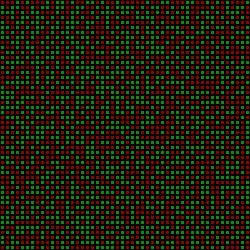
\includegraphics[width=0.25\textwidth]{boardi50_15}}%
            \hspace{8pt}%
            %
            \caption[]{Картины распределения спинов при $N=50\times 50$ для ферро- и антиферромагнетика.}%
            \label{fig:2}%
        \end{figure}
        %
        \begin{figure}[!htb]%
            \centering
            %
            \subfloat[][]{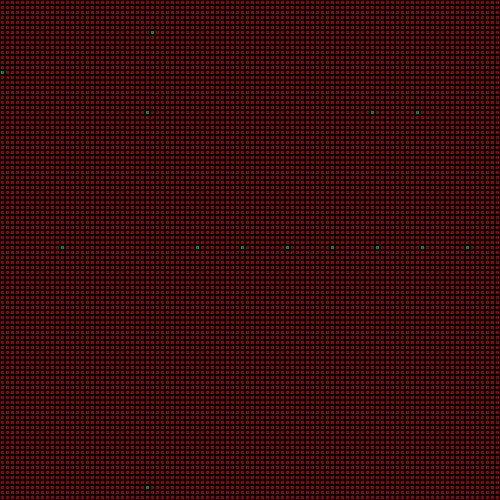
\includegraphics[width=0.25\textwidth]{board100_05}}%
            \hspace{8pt}%
            %
            \subfloat[][]{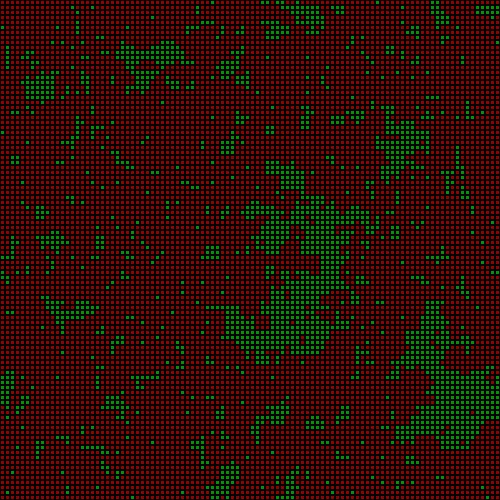
\includegraphics[width=0.25\textwidth]{board100_10}}%
            \hspace{8pt}%
            %
            \subfloat[][]{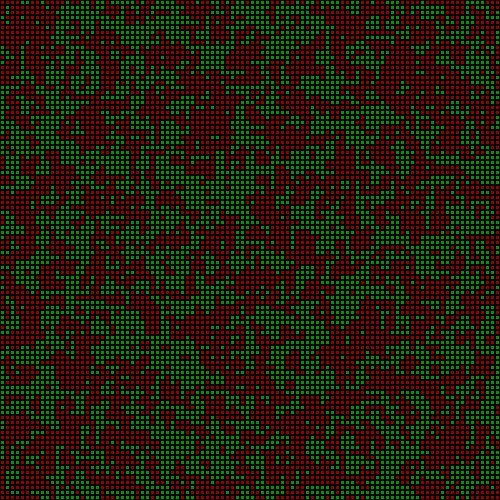
\includegraphics[width=0.25\textwidth]{board100_15}}%
            \hspace{8pt}%
            %
            \subfloat[][]{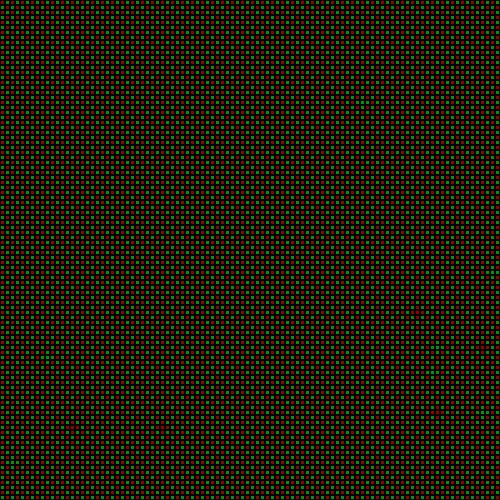
\includegraphics[width=0.25\textwidth]{boardi100_05}}%
            \hspace{8pt}%
            %
            \subfloat[][]{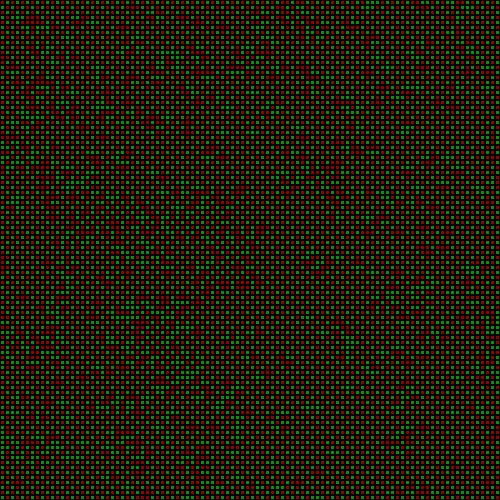
\includegraphics[width=0.25\textwidth]{boardi100_10}}%
            \hspace{8pt}%
            %
            \subfloat[][]{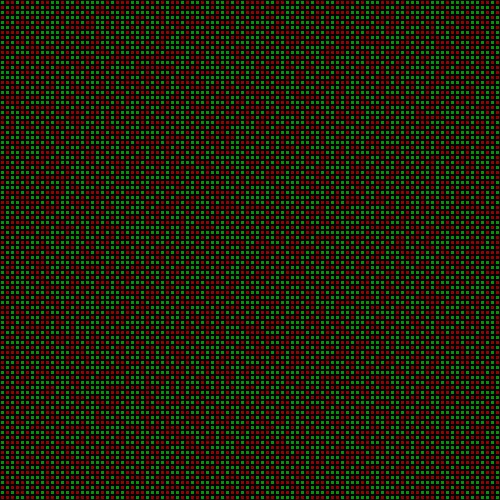
\includegraphics[width=0.25\textwidth]{boardi100_15}}%
            \hspace{8pt}%
            %
            \caption[]{Картины распределения спинов при $N=100\times 100$ для ферро- и антиферромагнетика.}%
            \label{fig:3}%
        \end{figure}
        %
        \begin{figure}[!htb]%
            \centering
            %
            \subfloat[][]{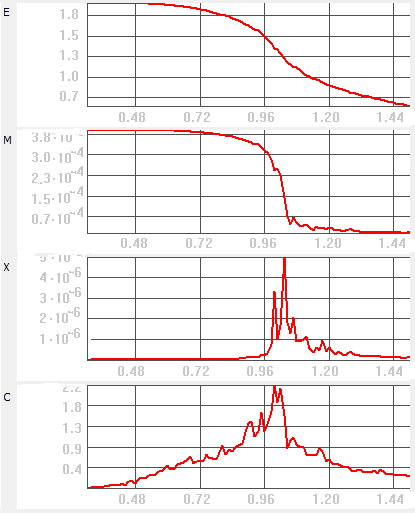
\includegraphics[width=0.4\textwidth]{plt}}%
            \hspace{8pt}%
            %
            \subfloat[][]{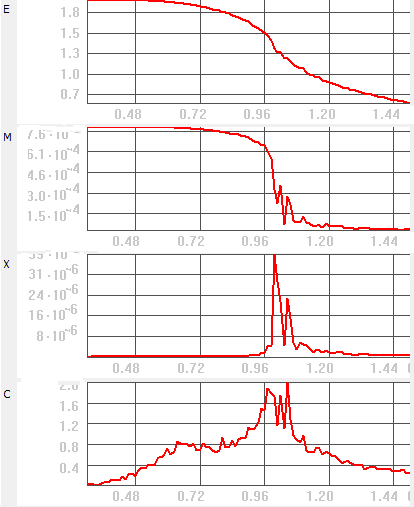
\includegraphics[width=0.4\textwidth]{plti}}%
            \hspace{8pt}%
            %
            \caption[]{Графики энергии, намагниченности, магнитной восприимчивости и теплоемкости для ферро- и антиферромагнетика при количестве спинов $N=50\times 50$. По графику теплоемкости (расположению максимума на нем) можно определить температуру фазового перехода. Она составила $0.98 T_c$ и $1.04 T_c$ соответственно.}%
            \label{fig:4}%
        \end{figure}

        С увеличением размеров области существенно возрастает вычислительная сложность алгоритма. Кроме того, скорость установления стационарного состояния существенно уменьшается. Это делает весьма сложным использование моделей уже с размером области моделирования более чем $500 \times 500$ для получения температурных зависимостей за приемлемое время.

        На \autoref{fig:4} изображены зависимости макроскопических параметров от температуры. Температура представлена в долях критической температуры $T_c$. Видно, что график энергии вблизи критической температуры имеет перегиб, а график теплоемкости в окрестности $T_c$ имеет максимум. Полученное по графикам значение $T_c$ весьма близко к теоретическому значению.

    %
    %
    %
    %%%%%%%%%%%%%%%%%%%%%%%%%%%%%%%%%%%%%%%%%%%%%%%%%%%%%%%%%%%%%%%%%%%%%%%
    %                           SECTION                                   %
    %%%%%%%%%%%%%%%%%%%%%%%%%%%%%%%%%%%%%%%%%%%%%%%%%%%%%%%%%%%%%%%%%%%%%%%
    %
    %
    %

    \section{Выводы}

        В ходе работы была написана демонстрационная программа, позволяющая исследовать динамику модели Изинга и получать макроскопические характеристики системы при разных температурах.

        При помощи полученной модели был смоделирован фазовый переход второго рода в ферро- и антиферромагнетике. Вычисленная температура фазового перехода оказалась близка к теоретической. Характерный вид зависимостей макроскопических параметров от времени также схож с известным для реальных ферромагнетиков.

    \clearpage

    \phantomsection
    \addcontentsline{toc}{section}{Список литературы}

    \nocite{*}
    \bibliographystyle{utf8gosttu}
    \bibliography{books}

\end{document}
